\documentclass[12pt,a4paper,fleqn]{article}
\title{Progress Report}
\author{Syed Ahmad Raza\\
        D10503816}
\date{2018.09.26}
\usepackage{mathtools}      % for math
\usepackage{graphicx}       % for graphics
%\usepackage{xcolor}         % for using colors in document
%\usepackage{afterpage}
\usepackage{float}          % force a figure placement with [H] command
%\usepackage{enumitem}       % control layout of itemize and enumerate
\usepackage{newtxtext}      % better text font
\usepackage{newtxmath}      % better math font
\usepackage{nicefrac}       % use nicer smaller fractions
%\usepackage{layouts}       % find \printinunitsof{in}\prntlen{\textwidth}
\graphicspath{{../figures/}}% only works when -shell-escape option is used

\begin{document}
\maketitle
\tableofcontents
\pagebreak

\section{Introduction}

In order to model fluid flow problems of interest, an in-depth knowledge of Finite Volume Method is essential. To model fluid flows for my research work, I have independently developed two-dimensional (2D) and three-dimensional (3D) solvers in C++. Results from the 2D and 3D solvers have also been validated using published research.

\section{Modeling Navier-Stokes equations using Finite Volume Method}

Continuity equation is
\begin{equation}\label{eq:continuity}
\nabla \cdot \mathbf{u} = 0 \quad,
\end{equation}
and Navier-Stokes equation is
\begin{equation}\label{eq:navier-stokes}
\frac{\partial \mathbf{u}}{\partial t}+\nabla \cdot (\mathbf{u}\mathbf{u}) = -\frac{1}{\rho}\nabla p + \nu \nabla^2 \mathbf{u}+\mathbf{f} \quad,
\end{equation}
where $\mathbf{u}$ is the velocity vector, \textit{p} is the pressure, $\rho$ is density of the fluid, and $\mathbf{f}$ is body force per unit mass.

Ignoring the body force $\mathbf{f}$, we are left with
\begin{equation}\label{eq:navier-stokes-no-f}
\frac {\partial \mathbf{u}}{\partial t} = -\frac{1}{\rho}\nabla p -\nabla \cdot (\mathbf{uu}) + \nu \nabla^2 \mathbf{u} \quad.
\end{equation}

Using a new vector $\mathbf{u}^*$ for intermediate velocity and \textit{n} as the index for time step, projection method is used to decompose Navier-Stokes equation in \eqref{eq:navier-stokes-no-f} into two parts,
\begin{equation}\label{eq:projection01}
\frac{\mathbf{u}^*-\mathbf{u}^n}{\Delta t} = -\nabla \cdot (\mathbf{u}\mathbf{u})+ \nu \nabla^2 \mathbf{u} \quad,
\end{equation}
which accounts for the convective and diffusive terms, and
\begin{equation}\label{eq:projection02}
\frac{\mathbf{u}^{n+1}-\mathbf{u}^*}{\Delta t}=-\frac{1}{\rho}\nabla p \quad,
\end{equation}
which accounts for the pressure term.

The equations were discretized and coded. The velocities in the diffusion terms were found using the second-order central scheme and the velocities in the convective terms were obtained using QUICK (Quadratic Upstream Interpolation for Convective Kinematics) scheme.

Euler scheme was utilized for the first time step and Adam-Bashforth scheme was used for the remaining. Denoting the terms on the right-hand side of equation \eqref{eq:projection01} with $\mathcal{F}(\mathbf{u})$, the second order Adams-Bashforth scheme can be applied using
\begin{equation}\label{eq:adams-bashforth}
\frac{\mathbf{u}^*-\mathbf{u}^n}{\Delta t} = \frac{3}{2}\mathcal{F}(\mathbf{u}^n)-\frac{1}{2}\mathcal{F}(\mathbf{u}^{n-1})\quad .
\end{equation}

Using the conservation of mass principle for the $n+1^{\text{st}}$ time step,
\begin{equation} \label{eq:continuity-n+1}
\nabla \cdot \mathbf{u}^{n+1} = 0 \quad ,
\end{equation}
and substituting equation \eqref{eq:projection02}, we get the Poisson equation for pressure
\begin{equation} \label{eq:poisson}
\nabla^2 p^{n+1} = \frac{\rho}{\Delta t}\nabla \cdot \mathbf{u}^* \quad .
\end{equation}

The Poisson equation for pressure is solved using successive over-relaxation method (SOR).

Finally, the correct velocity can be found using
\begin{equation}
\mathbf{u}^{n+1} = \mathbf{u}^* - \frac{\Delta t}{\rho}\cdot \nabla p^{n+1} \quad .
\end{equation}

\section{Results and validation of two-dimensional solver}

The 2D code was utilized to model the popular lid-driven cavity flow, which is commonly used to validate CFD solvers. The solver was used to obtain results for various uniform grid sizes and compared with the results of Ghia et. al \cite{GHIA1982387}. A velocity vector plot generated using ParaView is also shown below along with the validation results. All the cases were run for \(\text{Re}= 100\).

\begin{figure}[H]
    \centering
    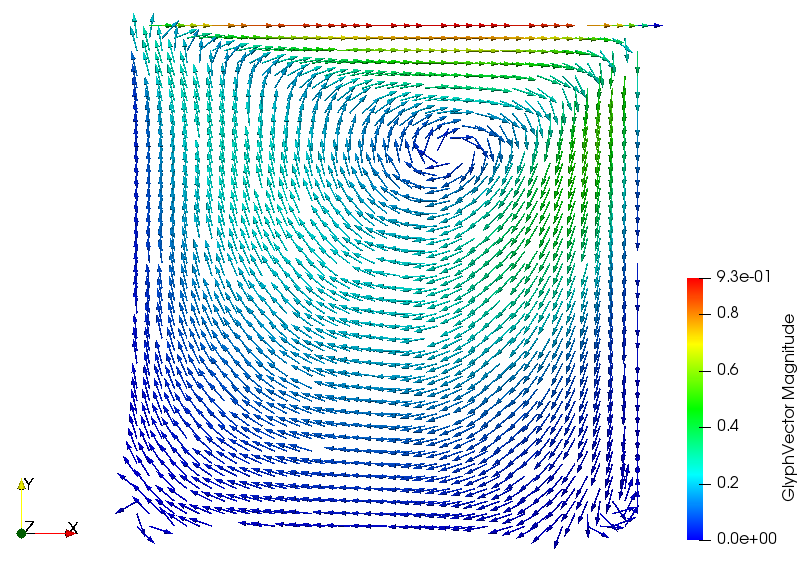
\includegraphics[width=\linewidth]{2DvelVectors.png}
    \caption{Velocity vectors plotted using ParaView for \(41 \times 41\) grid.}
\end{figure}

\begin{figure}[H]
    \centering
    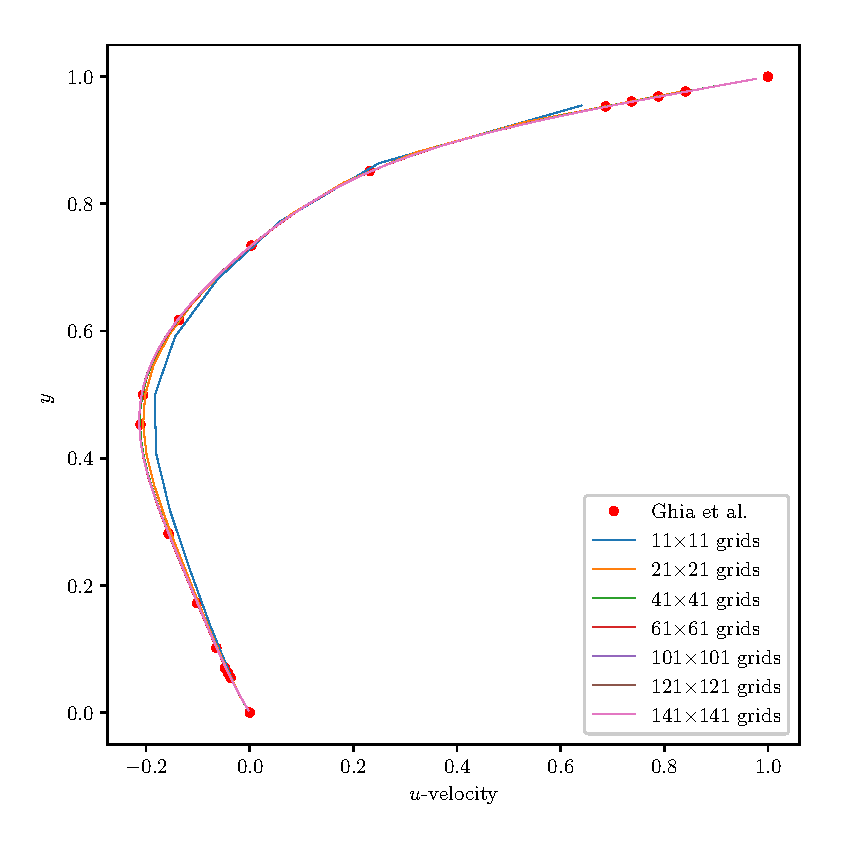
\includegraphics[width=\linewidth]{2Dfinal18051412_cavityFlowU.eps}
    \caption{\(x\)-direction velocities at the center of \(x\)-axis are plotted against \(y\)-coordinates for various uniform grid sizes, and their comparison with the results of \cite{GHIA1982387}.}
\end{figure}

\begin{figure}[H]
    \centering
    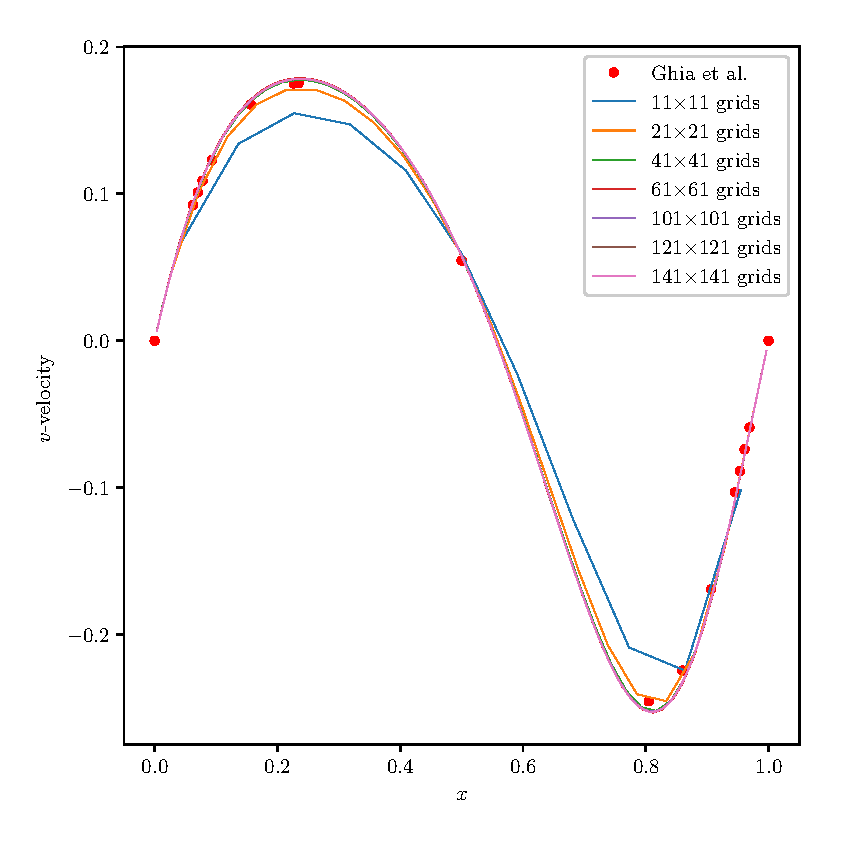
\includegraphics[width=\linewidth]{2Dfinal18051412_cavityFlowV.eps}
    \caption{\(y\)-direction velocities at the center of \(y\)-axis are plotted against \(x\)-coordinates for various uniform grid sizes, and their comparison with the results of Ghia et. al \cite{GHIA1982387}.}
\end{figure}

\pagebreak

\subsection{Unequal grid intervals}
Another grid with unequal grid intervals was used to test the code. The results, along with those of Ghia et. al for comparison \cite{GHIA1982387}, are shown in the figures below.

\begin{figure}[H]
    \centering
    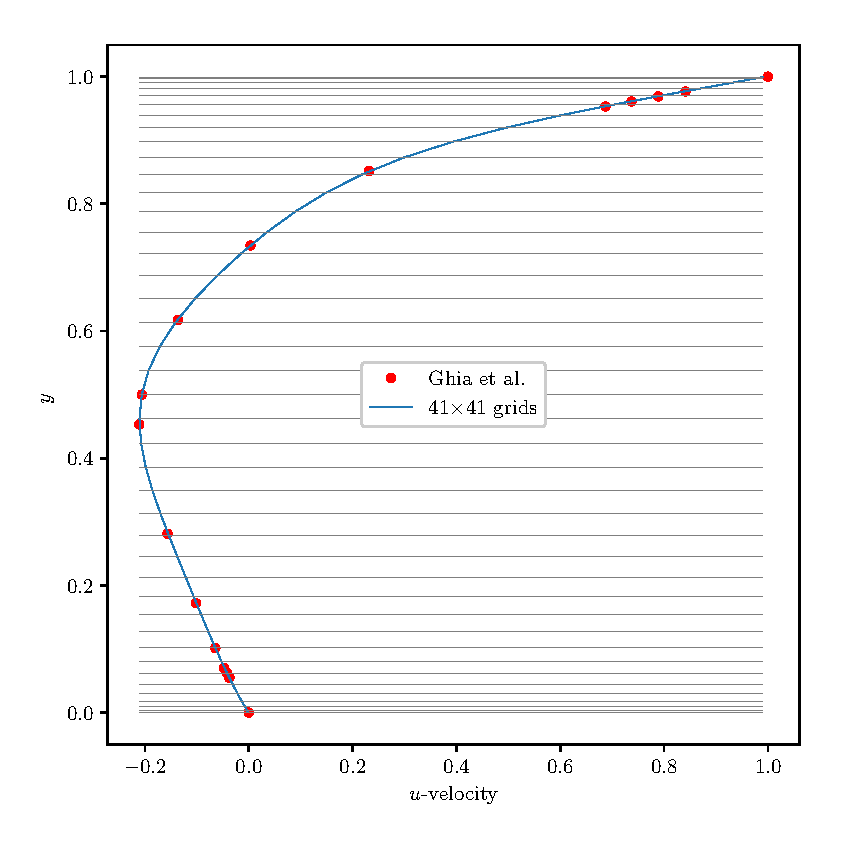
\includegraphics[width=\linewidth]{2Dunequal_cavityFlowU.eps}
    \caption{\(x\)-direction velocities at the center of \(x\)-axis are plotted against \(y\)-coordinates for unequal grid sizes, and compared with the results of Ghia et. al.}
\end{figure}

\begin{figure}[H]
    \centering
    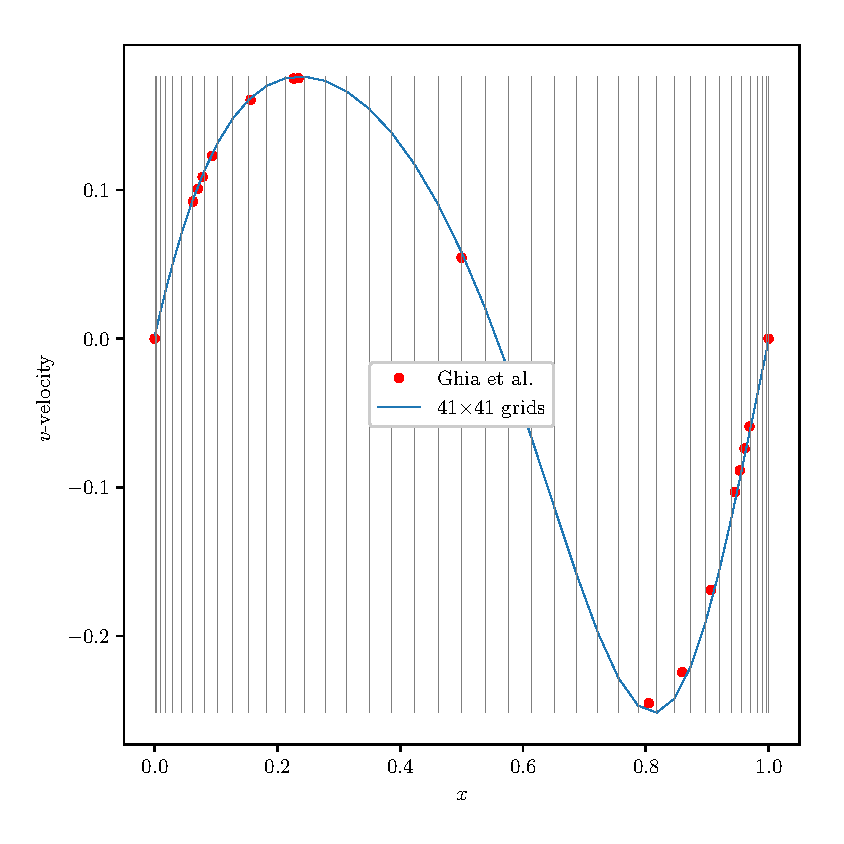
\includegraphics[width=\linewidth]{2Dunequal_cavityFlowV.eps}
    \caption{\(y\)-direction velocities at the center of \(y\)-axis are plotted against \(x\)-coordinates for unequal grid sizes, and compared with the results of Ghia et. al.}
\end{figure}

\section{Results and validation of three-dimensional solver}

The 3D solver was used to model a lid-driven cubic cavity flow for \(\text{Re}=100\). The pressure contours and velocity vectors for \(41 \times 41 \times 41\) grid size are shown below.

\begin{figure}[H]
    \centering
    \includegraphics[width=\linewidth]{3DPressure.png}
    \caption{Pressure contours in three-dimensional cavity flow for \(41 \times 41 \times 41\) grid size.}
\end{figure}

\begin{figure}[H]
    \centering
    \includegraphics[width=\linewidth]{3DVelVectors.png}
    \caption{Velocity vectors in three-dimensional cavity flow for \(41 \times 41 \times 41\) grid size.}
\end{figure}

\subsection{Comparison with published literature}
The simulation results at \(\text{Re}=100\) have been compared with the published results of Ku et al. \cite{Ku:1987:PMS:33136.33145} for three-dimensional cubic cavity flow and Ghia et al. \cite{GHIA1982387} for two-dimensional square cavity flow. The figures below represent the comparison of \(x\)-direction velocity \(u\) on the vertical centerline and \(y\)-direction velocity \(v\) on the horizontal centerline of the cubic cavity.

\begin{figure}[H]
    \centering
    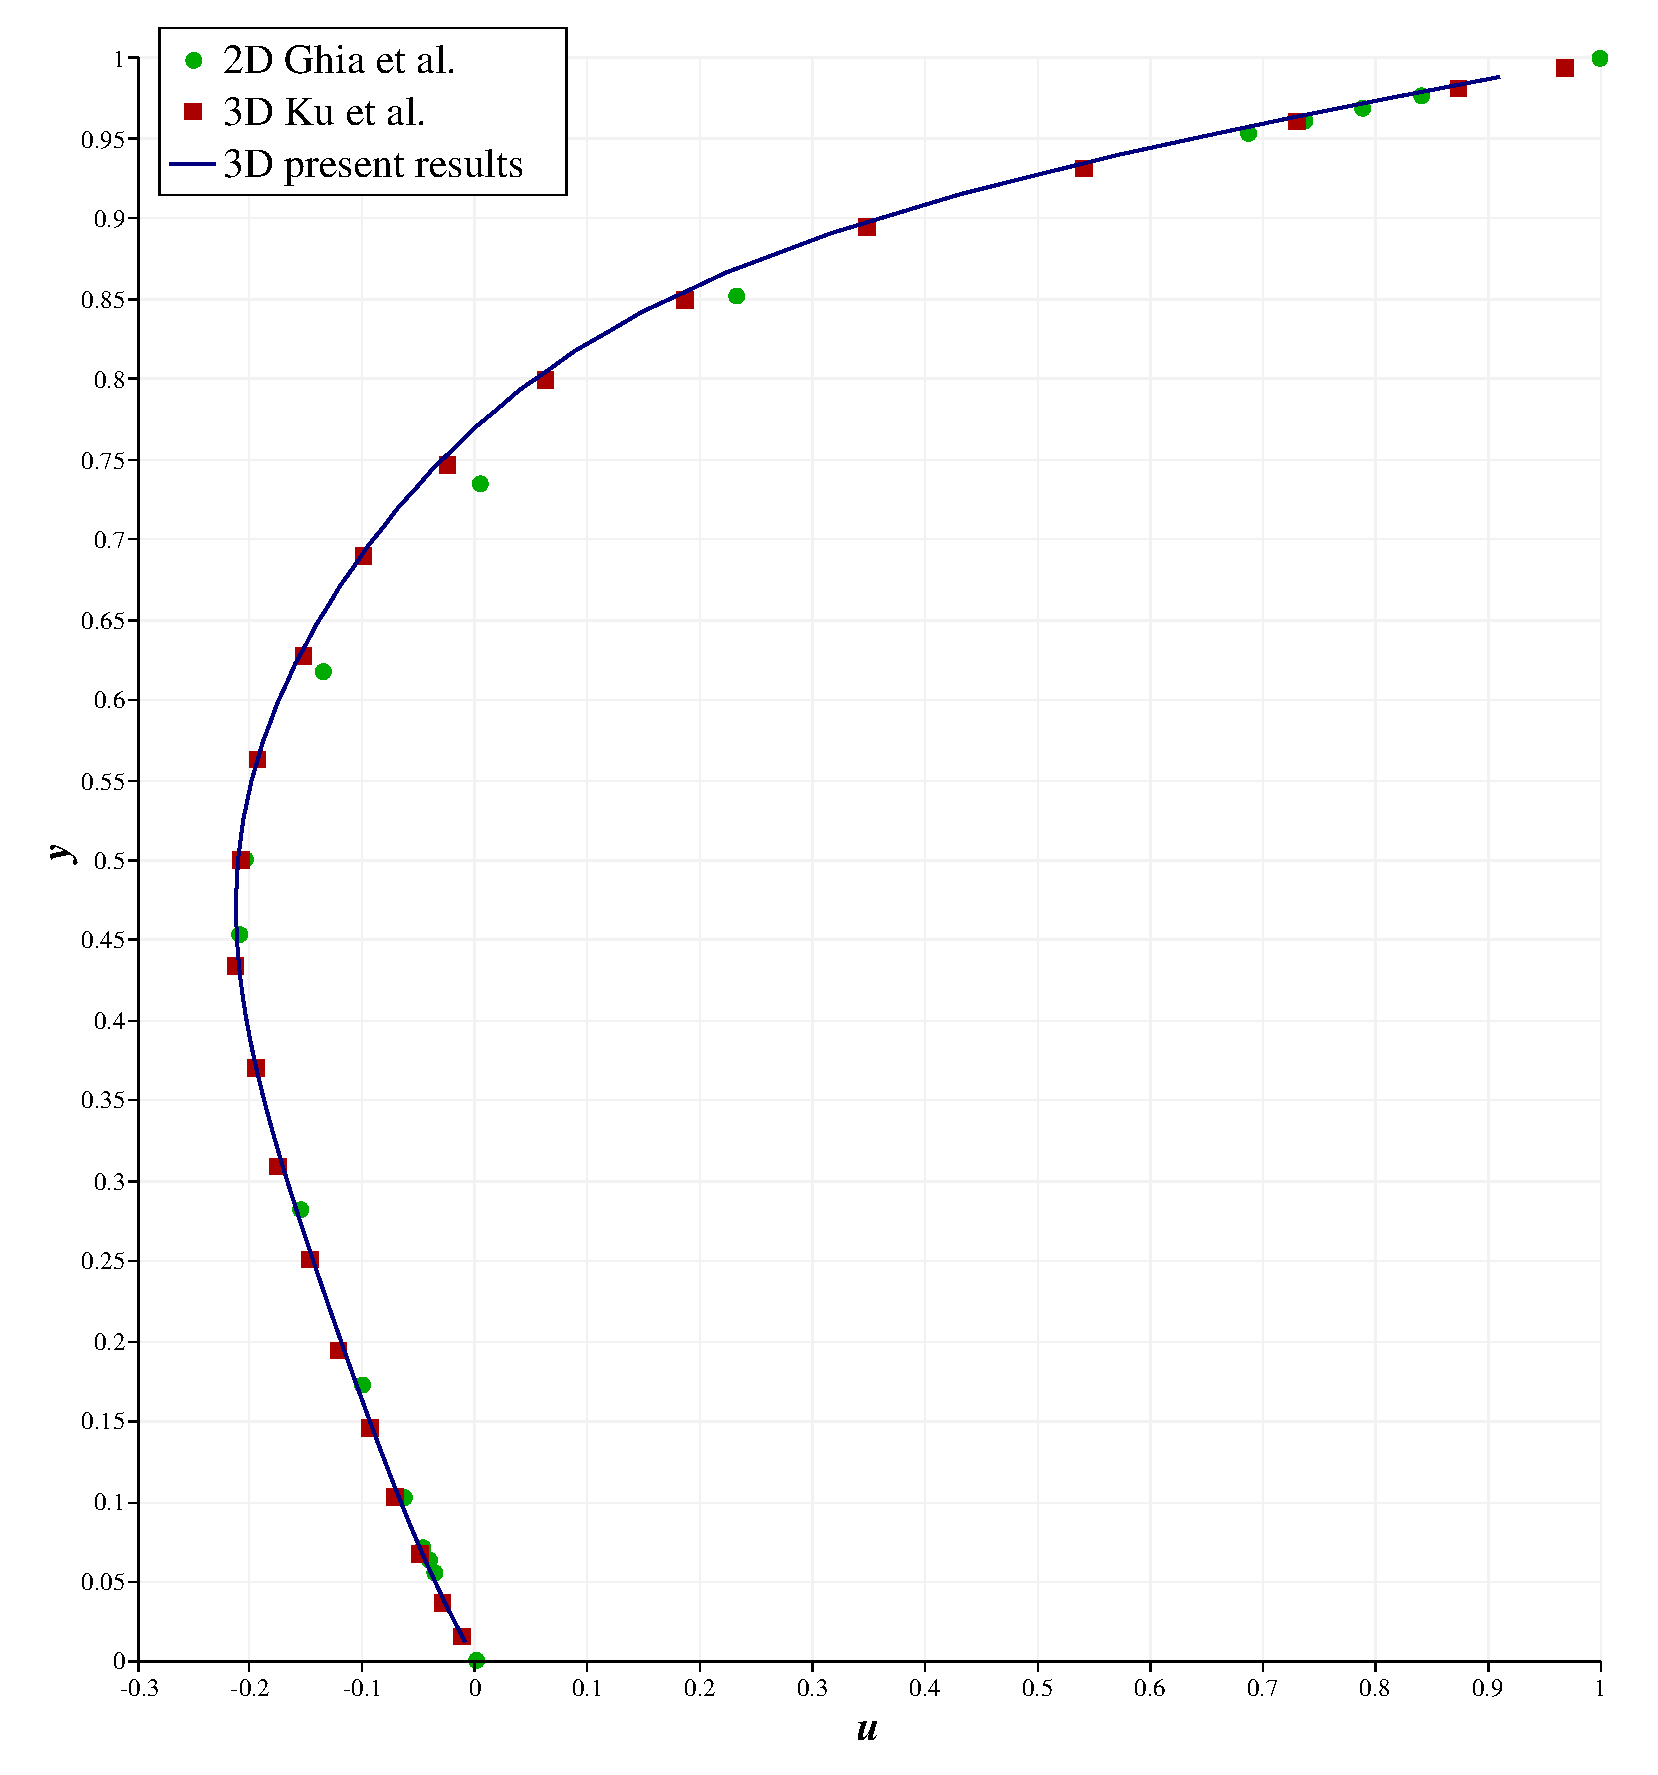
\includegraphics[width=\linewidth]{U-3D_vs_Ku-3D.eps}
    \caption{\(u\)-velocity profile on the vertical centerline in cubic cavity (at the center of \(z\)-axis).}
\end{figure}

\begin{figure}[H]
    \centering
    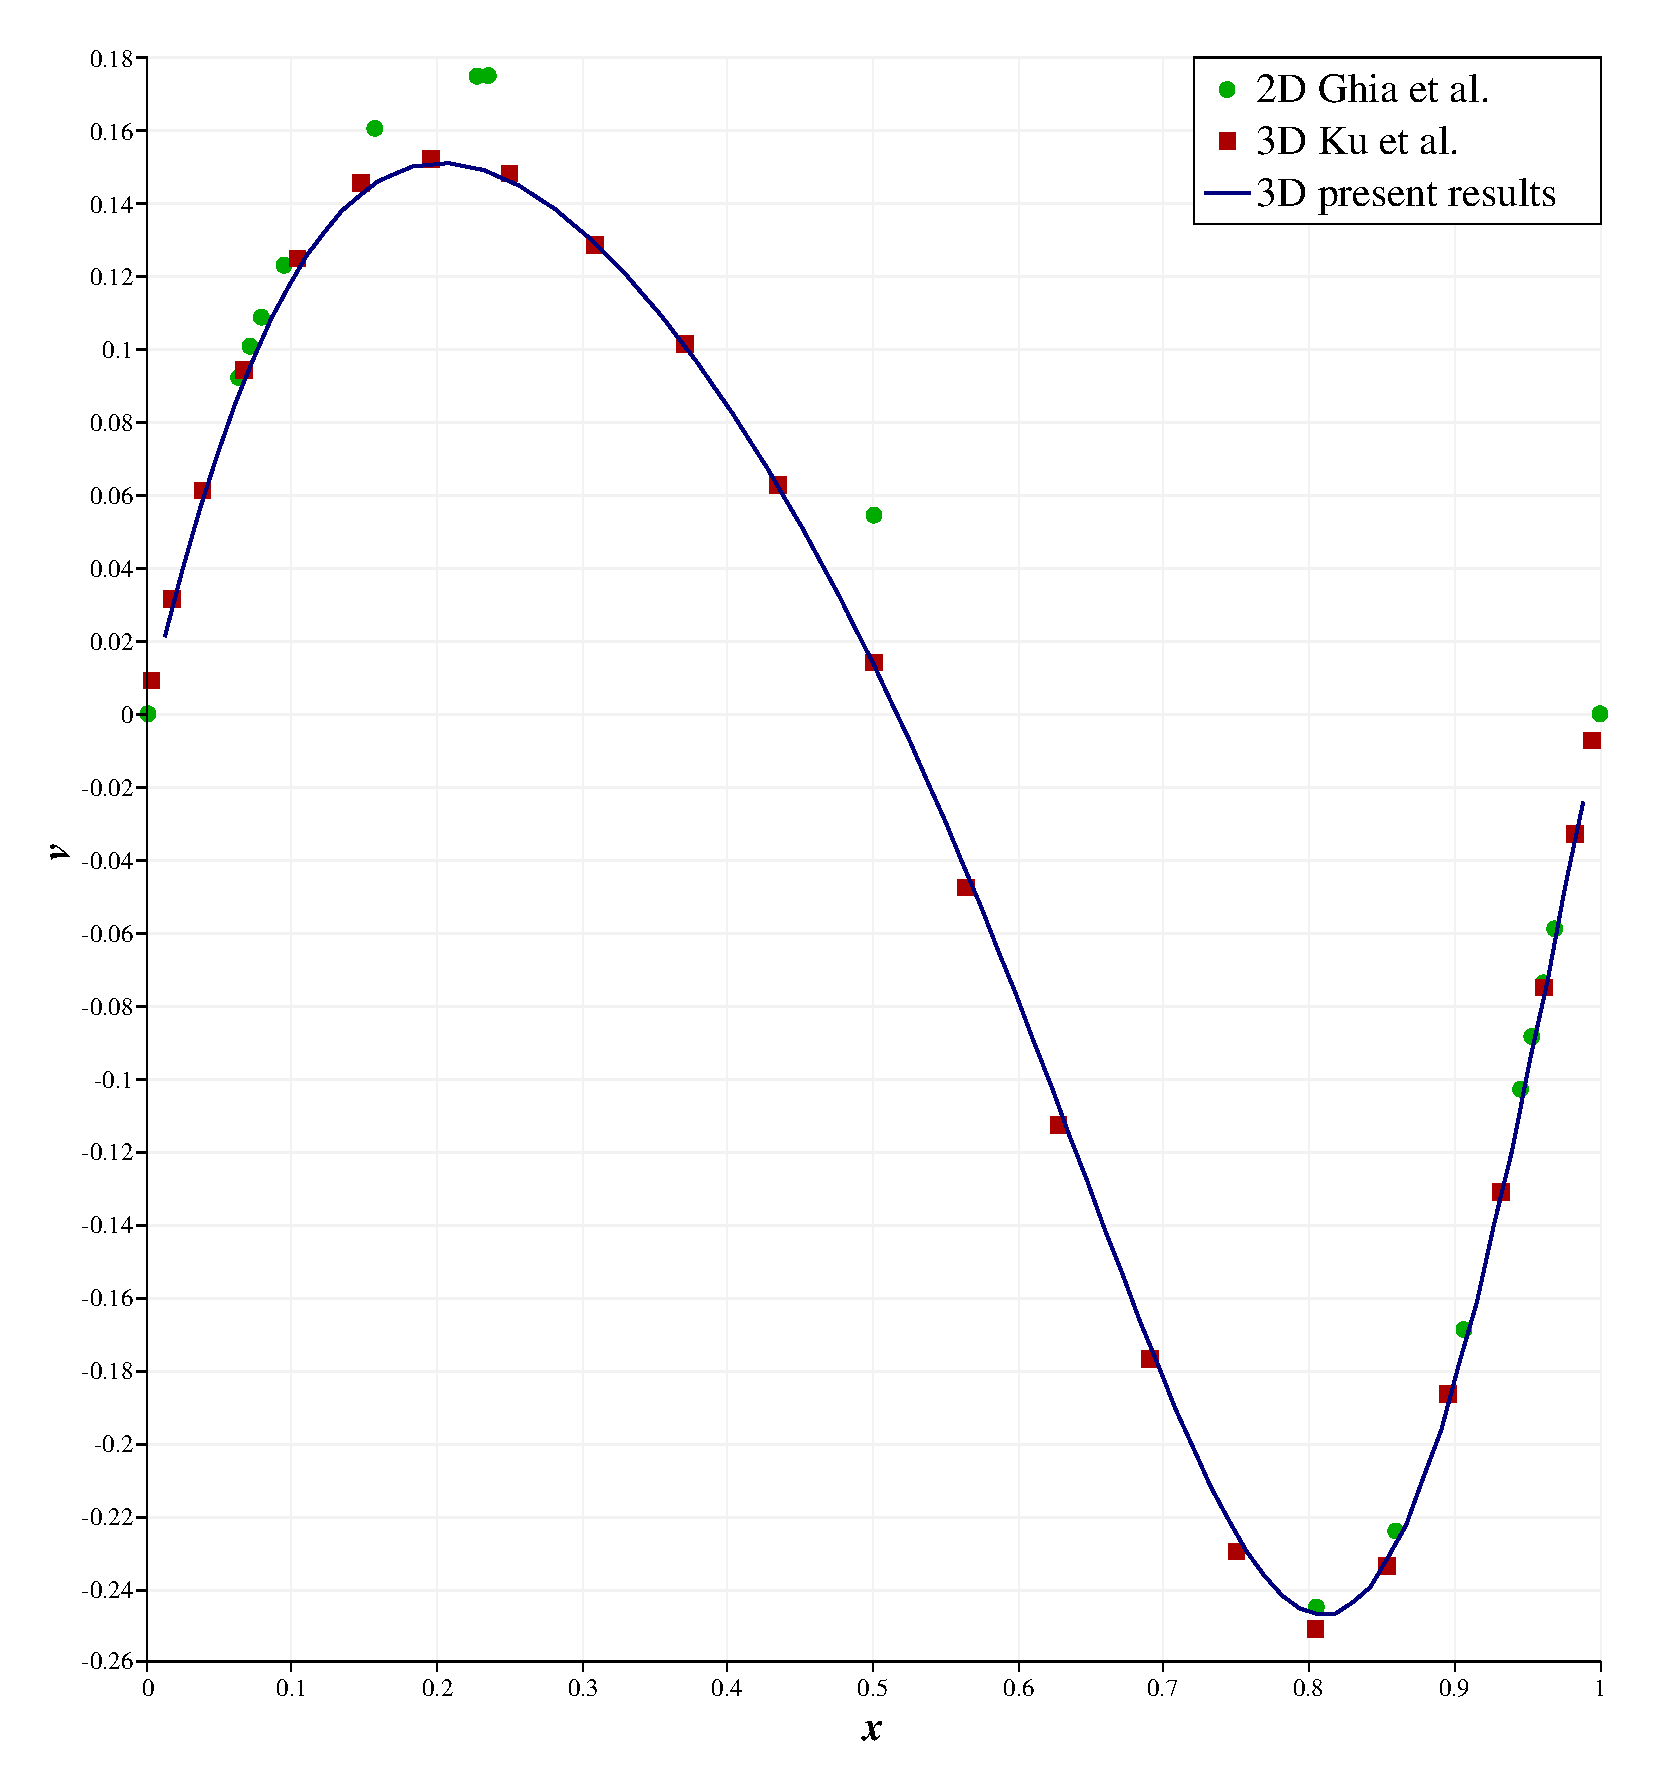
\includegraphics[width=\linewidth]{V-3D_vs_Ku-3D.eps}
    \caption{\(v\)-velocity profile on the horizontal centerline in cubic cavity (at the center of \(z\)-axis).}
\end{figure}

The results of the developed solver are in very good agreement with the three-dimensional results of Ku et al \cite{Ku:1987:PMS:33136.33145}. The differences with two-dimensional flow are apparent due to the effect of three-dimensional boundary conditions.

\bibliographystyle{unsrt}
\bibliography{33145.bib,0021999182900584.bib}

\end{document}
